\documentclass[11pt]{article}

\usepackage[utf8]{inputenc}
\usepackage[T1]{fontenc}
\usepackage{indentfirst}
\usepackage{titlesec}
\usepackage{listings}
\usepackage{float}

\titlelabel{\thetitle.\quad}

\renewcommand{\lstlistingname}{Programski odsječak}
\renewcommand{\figurename}{Slika}

%Gummi|063|=)
\title{\textbf{MapReduce}\\
		Raspodijeljeni sustavi - 2. domaća zadaća}
\author{Matija Šantl \\
		0036458898}
\date{}
\usepackage{graphicx}
\begin{document}

\maketitle

\section{Uvod}
Većina proračuna koje današnja računala obavljaju je poprilično jednostavno, ali zbog veličine ulaznih podataka, ti se proračuni moraju obavljati na raspodijeljenim sustavima koji sadrže stotine pa i tisuće računala kako bi ti proračuni završili u razumnom vremenu. Problemi poput paralelizacije proračuna, raspodijele podataka ili fizičkih kvarova računala bi mogli narušiti nadasve jednostavnu polaznu zamisao.

Rješenje tog problema je ponudila kompanija \emph{Google. Inc}. U sklopu tog rješenja razvijen je apstraktan model koji omogućava izražavanje jednostavnih proračuna te od korisnika drži skrivene detalje implementacije paralelizacije proračuna, raspodijele podataka, upravljanja fizičkih kvarova računala. Njihovo je rješenje inspirirano \emph{map} i \emph{reduce} primitivima programskog jezika \emph{Lisp}. 

Većina proračuna je uključivala provedbu neke funkcije nad podacima (operacija \emph{map}) kako bi se dobio skup podataka nad kojim se provodi operacija redukcije (\emph{reduce}) nad istoimenim elementima. Korištenje modela funkcijskog programiranja s operacijama \emph{map} i \emph{reduce} definiranim od strane korisnika olakšalo je paralelizaciju velikih proračuna.

Najveći doprinos ovakvom rješenju je jednostavno i moćno sučelje koje omogućuje automatiziranu paralelizaciju i distribuciju proračuna velikih razmjera kombinirano s implementacijom tog sučelja koje postiže visoke performanse na velikim grozdovima osobnih računala.

\section{MapReduce}
Ulazni i izlani podaci se mogu predočiti kao skup ključ/vrijednost parova. Korisnik \emph{MapReduce} biblioteke izražava proračune pomoću funckija \emph{Map} i \emph{Reduce}.

\emph{Map} funckija, koju je napisao korisnik, kao ulaz prima jedan par i kao rezultat vraća skup ključ/vrijednost parova. \emph{MapReduce} biblioteka tada grupira zajedno sve vrijednosti koje imaju isti ključ i prosljeđuje ih \emph{Reduce} funkciji.

\emph{Reduce} funckija, koju je također napisao korisnik, kao ulazni parametar uzima ključ i skup vrijednosti koje pripadaju tom ključu. Dobivene vrijednosti spaja tako da se na izlazu može pojaviti skup s manjim brojem članova nego ulazni. Uobičajeno je da \emph{Reduce} vrati najviše jednu vrijednost. 

\subsection{Tipovi}
\emph{Map} i \emph{Reduce} funkcije su definirane na sljedeći način:

$$map(k1,v1) \rightarrow  list(k2,v2)$$
$$reduce(k2,list(v2)) \rightarrow  list(v2)$$

To znači da se domene ulaznih ključ/vrijednost parova različite od izlaznih domena ključ/vrijednost parova. Izvorno programsko ostvarenje u C++ programskom jeziku prosljeđuje \emph{String} tip podataka te ostavlja korisniku da radi pretvorbe u konačni tip podatka.

\subsection{Primjer}
Promatrajmo problem brojanja pojavljivanja riječi u velikom skupu dokumenata.

\emph{Map} funkcija bi mogla od svake riječi napraviti par gdje je ključ sama riječ a vrijednost broj 1. \emph{Reduce} funkcija bi tada sumirala sve vrijednosti s istim ključem tj. ista riječ, te bi tako na kraju za svaku riječ dobili broj pojavljivanja u dokumentu. 

Ilustracija postupka nad primjerom dana je na slici \ref{primjer}.
\begin{figure}[H]
\centering
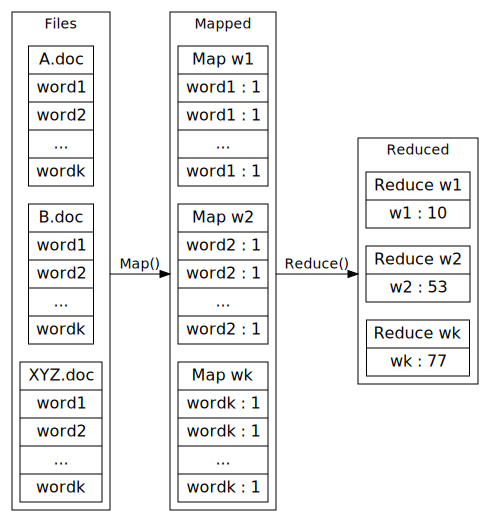
\includegraphics[scale=0.3]{ilustracija.png}
\caption{Primjer \emph{MapReduce}}
\label{primjer}
\end{figure}

Moguće programsko ostvarenje je prikazano u programskom odjsečku \ref{map} i \ref{reduce}.
\begin{lstlisting}[caption=Funkcija Map, label=map]
map(String key, String value): 
	// key: document name 
	// value: document contents 
	for each word w in value: 
		EmitIntermediate(w, "1"); 
\end{lstlisting}

\begin{lstlisting}[caption=Funkcija Reduce, label=reduce]
reduce(String key, Iterator values): 
	// key: a word 
	// values: a list of counts 
	int result = 0; 
	for each v in values: 
		result += ParseInt(v); 
	Emit(AsString(result)); 
\end{lstlisting}

\section{Primjena}
Prva verzija \emph{MapReduce} bibilioteke je nastala u veljači 2003. godine te su do kolovoza 2003. napravljena znatna poboljšanja u pogledu performansi poput lokalne optimizacije i dinamičkog raspoređivanja posla. Nakon toga je \emph{MapReduce} model uvelike prihvaćen za rješavanje raznih problema  u područjima poput:
\begin{itemize}
\item strojno učenje
\item grupiranje (\emph{clustering})
\item dubinsko pretraživanje podataka (\emph{data mining})
\item teorija grafova
\end{itemize}

\section{Zaključak}
MapReduce je model programiranja i pripadajuća izvedba za obradu velikih skupova podataka. Korisnik obabere funkciju mapiranja (\emph{Map}) koja obrađuje ključ/vrijednost parove kako bi generirala neposredan skup ključ/vrijednost parova, i funkciju reduciranja (\emph{Reduce}) koja onda spaja sve neposredne vrijednosti koje su povezane s istim ključem. 

Programi koji su pisani koristeći ovakav funkcijski stil se automatski paraleliziraju i mogu se izvršavati na velikim grozdovima računala. Sustavi za pokretanje brinu oko detalja poput raspodijele ulaznih podataka, raspoređivanja izvršavanja na skupu raspodijeljenih računala, nošenje s fizičkim kvarovima računala i komunikacije među računalima. To omogućava programerima bez puno iskustva s paralelnim i raspodijeljenim sustavima da lako iskoriste sve pogodnosti koje nude veliki raspodijeljeni sustavi.

Mnogi problemi iz stvarnog svijeta se mogu svesti na ovakav model, te je zbog toga ovaj model veoma primjenjivan u praksi.

\end{document}
